
\subsection{Tacit bidder collusion}
There is another kind of "collusion" apart from the explicitly agreed upon. This is "tacit" collusion where bidders use the market mechanism to signal their willingness to game the system. This is typically something that happens in repeated auctions or multi-unit auctions where the benefits of winning can be split evenly between market participants. Often tacit collusion is \textit{not} illegal, as the bidders simply exploit the auction rules set up by the seller. Amongst others the following characteristica of an auction can lead to tacit collusion:
\begin{itemize}
    \item \textbf{Transparency} when bids are transparent bidders get the opportunity to use their bids as signals encouraging tacit collusion.
    \item \textbf{Divisibility} When gains are easily divided bidders dont have to come up with an external mechanism to divide the profit (which would be illegal). 
    \item \textbf{Repeated interaction} if bidders can get to know each other they will recognize each others subtle signals.
    \item \textbf{Low uncertainty} if bidders are certain of the market circumstances they escape the uncertainty of their opponents capability to bid to marginal costs. 
    \item \textbf{Number of bidders} few bidders reduces the chance that one bidder breaks the tacit collusive equilibria.
    \item \textbf{Pricing mechanism} the second price mechanism is more vulnerable to collusion (why?)
\end{itemize}

\subsection{Cases from Denmark}
An example of tacit collusion by two suppliers of aspirin is shown in figure \ref{fig: medprices}.
\begin{SCfigure}[][h]
    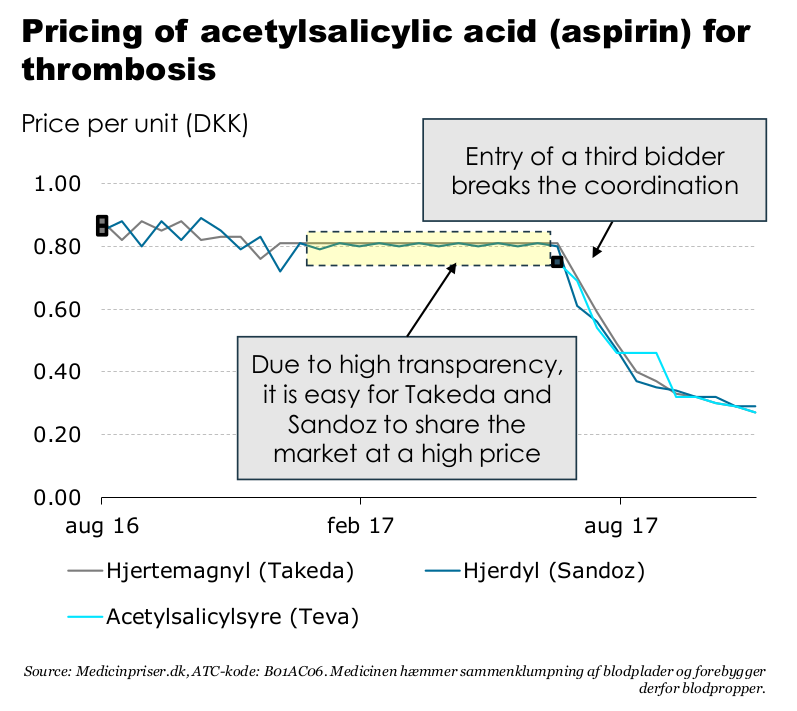
\includegraphics[width=0.6\textwidth]{figures/medprices.png}
    \caption{\textbf{Danish medicine prices} showing clear signs of tacit collusion.}
    \label{fig: medprices}
\end{SCfigure}

An example of an illegal coordination is how danish construction firms used to share bids in advance of auctions, so that companies could bid a reasonable but non-winning bid even though they didn't have the capacity to undertake the construction work. This practice was known in the industry as "keeping the customer warm", i.e. signalling that a construction company was still interested in future work, without revealing their capacity limits to the buyer. 

\subsection{Introduction to multiunit auctions}
The multiunit auctions are distinct from sequential auctions as they assume multiple units of the same item is auctioned away at once. Denote the number of units for sale $K$, each bidder submits a bid vector $b^i=(b_1^i, b_2^i, ..., b_K^i)$ which gives the willingness to pay for each item, assuming they have won all of the previous units. We can think of the bid vector as an \textit{inverse demand function}.
\\ \\
In this setting the previously studied auction formats can no longer be applied directly, instead the possible formats are 
\begin{itemize}
    \item Sealed bid discriminatory.
    (Bidders pay the sum of their winning bids)
    \item Sealed bid uniform price 
    (Bidders pay a fixed price times the number of items they win. The price is set as the clearing price which makes the demand equal supply)
    \item The Vickrey auction (also sealed)
    (Bidders pay equal to the bids they "push out" of the winning bids, note this collapses to the second price auction when $K=1$).
    \item The open bid Dutch 
    \item The open bid English 
    \item The Ausubel auction (also open)
\end{itemize}

\paragraph{Example (sealed bid)} consider the three bidders $A,B,C$ who submit bids as in figure \ref{fig: multiexample}. Each row here corresponds to a bid vector $b^A, b^B, b^C$. All of the above formats solve the problem of allocating all of the 6 units to the bidders with the highest bid, but differ in which prices are paid for each unit. 

\begin{SCfigure}[][h]
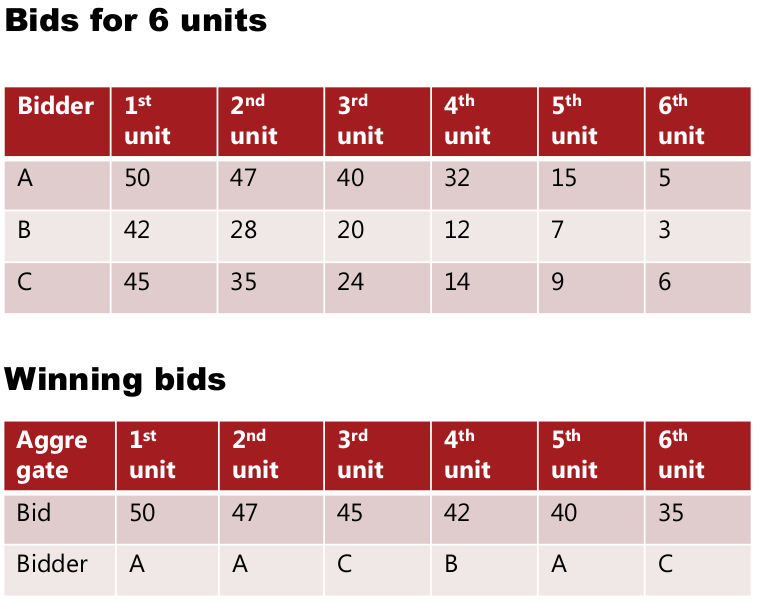
\includegraphics[width=0.6\textwidth]{figures/multibids.png}    
\caption{\textbf{Multi unit auction} example bids.}
\label{fig: multiexample}
\end{SCfigure}  

This auction will have winning bids also shown in figure \ref{fig: multiexample}. (We were shown how to calculate the prices on the blackboard).

\subsection{The day-ahead market in Northern Europe}
An example of a multiunit market is the day-ahead market for energy supply in Northern Europe. Here every hour of the following days electricity supply is auctioned away to suppliers. This is an example of a market which can produce "residual monopolies".
\\ \\
This auction is held as a uniform price auction, and so it might be benefitial to engage in demand reduction ("strategic capacity withholding"), see lecture 11.